\begin{figure*}[th]
\begin{center}
   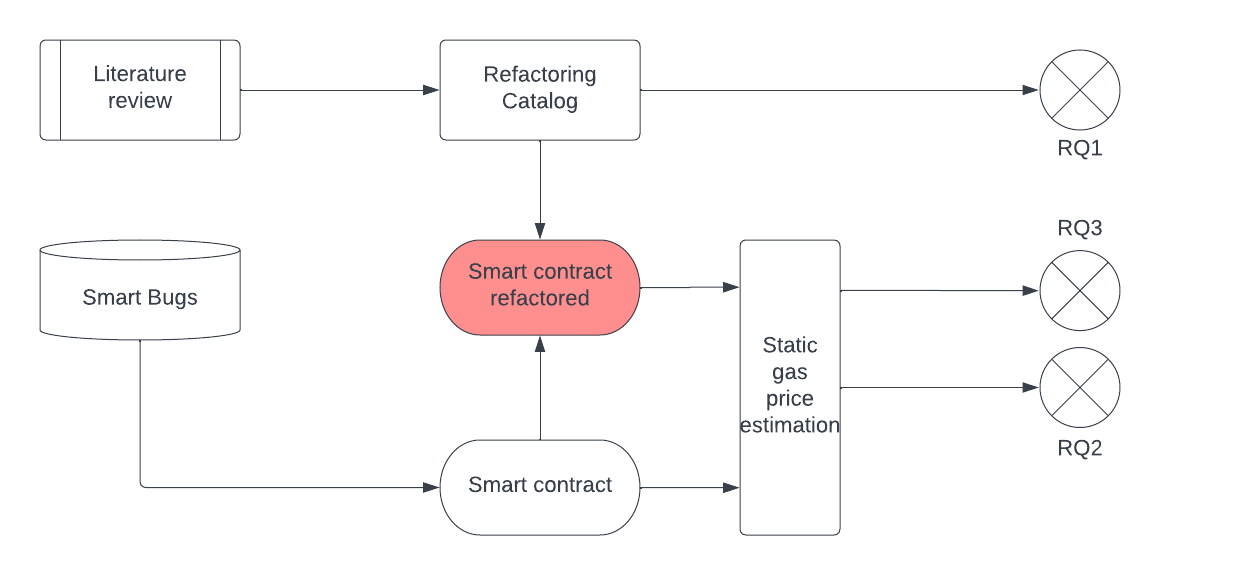
\includegraphics[scale=0.45]{figure/Impact of Code Refactoring on Gas Price.png}
   \caption{\label{fig:1}Overview of the study method}
\label{test_extraction}
\end{center}
\end{figure*}

\label{sec:Analysis Methodology}


 \emph{\\RQ1:\RQOne}
 
 

 \emph{\\RQ2:\RQTwo}
 


 \emph{\\RQ3:\RQThree}
 

 

\subsection{Data collection}
\label{sec:Data collection}

Smart Bugs : https://github.com/smartbugs/smartbugs-wild/tree/master/contracts








\subsection{Data Processing}
\label{sec:Data Processing}
In this sub-section, we describe the details of the data collection and analysis approach followed to answer our different research questions. This approach is depicted in Figure \ref{fig:1}. In the following, we elaborate on each data processing step.



\begin{enumerate}
  % \item \emph{Creation d'un code de simulation de déploiment avec tebderly:}(https://docs.tenderly.co/simulations-and-forks/simulation-api) ou ganache (https://www.youtube.com/watch?v=fH4KUgQCS7c&ab_channel=BenBK)
  
  \item \emph{Collecter et trier les Smart contract:}
  
  \item \emph{Mesurer le prix du gaz de chaque Smart contrat:}
  https://github.com/paperSubmition2020/GasmetReplicationPackage

  
  \item \emph{Inserer des modifications (aléatoirement - manuellement):}
  
  \item \emph{Documenter les modifications:}


  \item \emph{Mesurer le prix du gaz des smart contrats modifés:} 
  
\end{enumerate}




\subsection{Replication Package}
\label{sec:Replication Package}
